\chapter{Design}

In this chapter, we will describe the structure of the application, the problems that it has to face and the decisions we made to overcome those problems.

\section{Application architecture}

Our application is intended to be used on mobile devices. Due to this fact, we only have two different reasonable options of what application structure to use. We could either implement all of the functionality inside the mobile app, or split some of it into a server and use a client/server architecture. In our case, the decision to choose a client/server architecture was relatively straightforward due to the following reasons:

\begin{itemize}
    \item As we'll see later, the application works in 2 stages - it first parses the necessary data into memory and then performs the searches using this data. The parsing stage is computationally intensive, as the amount of data used is relatively large. On this large dataset, intensive computations need to be performed, such as computing all transfers and their lengths, calculating bike routes between bike stations or creating Route and Trip objects by merging data from the \texttt{trips.txt}, \texttt{stop\_times.txt}, \texttt{calendar.txt} and \texttt{calendar\_dates.txt} files. This operation takes a relatively long time (typically tens of seconds). When running the app on the server, this is not an issue, as this step is only performed once when launching the app and the parsed data can be used quickly and efficiently afterwards. However, if the app were to run solely on the mobile device, it would either need to be running in the background non-stop, which is very impractical and close to impossible on modern mobile operating systems, or it would need to perform this task every time the app was opened, which would make it very impractical to use

    \item During the parsing stage and when updating delay and bikesharing data, the application also needs to download large amounts of data from the web. This is not a problem when running the application on the server, but would cause heavy data consumption on the mobile device, where internet access may be expensive.

    \item The application also accesses publicly accessible APIs, which are not intended to be directly accessed by each client separately. Running the app on every client's device may cause these APIs to be overloaded with unnecessary requests. This can easily be prevented by only running the request once from the server and then further distributing the data among our users.

    \item If all the functionality was implemented for mobile devices, it would be necessary to implement the app at least twice to support both major mobile operating systems (Android and iOS), which can be prevented by implementing the main functionality for the server side once and only having to implement a light client application in two versions.
\end{itemize}

\subsection{Server-side responsibilities}

The server side implements all of the main routing functionality. It contains an API that accepts requests from the client. It processes all these requests by calculating and returning the best connections according to the request's parameters. In particular, it handles requests for new connections, requests for expanding the list of resulting connections to earlier or later ones, requests to find earlier or later alternatives for a particular trip and requests to update the delay information of existing connection results. 

\subsection{Client-side responsibilities}

The client is designed to be as simple as possible. Its only responsibilities are gathering user input and storing the user's preferences, sending requests to the server's API according to the input and preferences, parsing the results returned from the API and displaying them in a clear way to the user. The application is designed so that the developer implementing the client does not need any information on the inner workings of the server-side application. This is to ensure separation of concerns and also to make it easier to develop clients for multiple different platforms more easily.



\section{Programming language selection}
\label{subsec:programming_language}

\subsection{Server}

The main qualitative requirements that we have for the server-side application are for it to run as quickly and efficiently as possible and also to be easy to implement, maintain and extend the application. We selected the C\# programming language thanks to its combination of both of these qualities - its efficiency is comparable to other languages like C++ or Java and it provides both an extensive standard library for generic tasks such as performing HTTP requests or implementing a simple API with POST endpoints and an extensive selection of third-party libraries for more specific tasks we will need to perform, like routing using Open Street Maps data or parsing the Protocol Buffer files containing public transit delay data. A .NET application is also easily portable between different platforms should we need to run or test it in a different environment than the one it will normally run in. Another great benefit of using C\# as our programming language is its extensive and up-to-date official documentation.

\subsection{Client}

As explained earlier, due to its prevalence among users in the Czech Republic, we chose to implement the client for the Android operating system. While there are many different languages and frameworks with which it is possible to implement a native Android application, we ultimately decided on using the Kotlin programming language, particularly its Jetpack Compose toolkit for developing user interfaces. It is a tool maintained and supported by Google, Android's developer, with a very intuitive support for creating modern-looking UI components and communicating with the operating system. It also has great support in the official IDE for Android development, Android Studio.


\section{Algorithm design}

In this section, we will go over the problems that our application will need to solve, the different approaches that were possible and the decisions we made regarding the algorithms used. As the client side only implements very minimal functionality and mostly serves as a way to display the results, this section will only be concerned with the problems faced by the server-side application.

\subsection{Public transit routing}
\label{subsec:public_transit_routing}

The main problem our application is designed to solve is routing within a public transit network. A public transit network can essentially be described as a graph with stops as the vertices and trips, transfers and (in our case) bike trips as the edges.  However, there is one major catch. As opposed to a normal graph, traversing the edges corresponding to public transit trips is only possible at certain times using certain trips. This property of the network essentially prevents us from using any standard shortest-path graph algorithm, as they only account for the weights of the edges (the duration of the trip), but not for the edges only being "accessible" at certain times (i.e. the trips between them only operating on discrete times). 

However, this issue can be solved by partly modifying standard graph algorithms to account for this property of public transit networks, and so it would still theoretically be possible to use them for this purpose. So, let's go over some of them and their benefits and disadvantages:

\begin{itemize}
    \item \textbf{Dijkstra's algorithm} finds the shortest path from a source vertex to all other vertices, but the algorithm can be terminated after reaching the target\cite[pp. 146--152]{mares2017pruvodce}. When using Dijkstra's algorithm, the weights of the edges may only be positive or zero, but this is not an issue for our application, as in our case, the weights represent the time it takes to travel between the 2 vertices, which can clearly never be negative. The main issue with this algorithm is its nature in exploring vertices in all directions uniformly, which typically means that we reach the target vertex only after processing many irrelevant vertices in the opposite direction. Due to this, this algorithm is typically not very efficient in public transit networks. Detailed information on Dijkstra's algorithm can be found in \textcite[pp. 146--152]{mares2017pruvodce}.

    \item \textbf{A* algorithm} is a variation on Dijkstra's algorithm. Instead of uniformly exploring vertices in all directions, it applies a heuristic to prioritize exploring vertices in the direction of the target stop. This feature makes it a good fit for public transit application, as it generally is the case that the best connections between two stops more or less follow the straight-line between the 2 stops and generally do not wander off much in the opposite direction. More details on A* and its comparison with Dijkstra's algorithm can be found in \textcite[pp. 156--160]{mares2017pruvodce}.

    \item \textbf{Floyd-Warshall algorithm} is able to find the shortest distances between all pairs of vertices within the graph. Along with this, its other benefit is being able to handle graphs with negative edge weights\cite[pp. 154--155]{mares2017pruvodce}. However, as we already described above, this is useless for our use case and it thus makes no sense to select this less efficient algorithm over Dijkstra's or A* algorithms. The same is true of its ability to find the shortest path between all pairs of stops - that is a functionality we do not need a connection planning application to have, as there will always be one source and one destination point. Furthermore, the shortest path varies depending on the specified departure (or arrival) time, and thus this algorithm cannot be used to pre-calculate all the paths within the network. Thus, this algorithm's benefits over Dijkstra do not outweight the worse performance. More details on Floyd-Warshall's algorithm can be found in  \textcite[pp. 154--155]{mares2017pruvodce}
    
    \item \textbf{Bellman-Ford algorithm} is an alternative to Dijkstra's algorithm, finding the minimum distance to all other vertices within the graph as well. As opposed to Floyd-Warshall, it can also handle graphs with negative cycles. However, once again this is a feature we do not need, and as it is also slower than Dijkstra's algorithm\cite[pp. 152--153]{mares2017pruvodce}, it does not fit our use case.
\end{itemize}

As we can see from this comparison of known graph algorithms, it seems that our best option is to use the A* algorithm. And that is what many public transit routing applications actually use. However, there is also one more option. A new algorithm called \textbf{RAPTOR} (Round-bAsed Public Transit Optimized Router), targeted specifically at solving the public transit connection search problem was developed by Microsoft's research team in 2012\cite{delling2015raptor}.

This algorithm takes advantage of the fact that it is designed for this exact setting and uses the fact that the edges within the graph are grouped into routes and trips. As the name suggests, it works in a finite number of rounds. In principle, it initiates the search by setting the best reach time of all stops to the worst bound except the start stops, where it sets it to the departure time set by the user. It holds a set of marked stops, to which it adds these starting stops. After that, the algorithm itself begins. 

In every round, it first accumulates all routes that pass through any marked stop. The stop will be considered its boarding point. If a route passes through multiple marked stops, it takes the first one (in order) as the boarding point. After this, for every one of these marked routes, it first finds the first trip on that route that departs the boarding point after the best current reach time there. Then, it traverses the trip, meaning it relaxes reach times at all the following stops according to the time the trip gets there and marks them. If it reaches a stop that was already reached at a better time, it again has to find the earliest trip of this route that departs the stop after its best reach time. This may be the same trip, or it might actually be a better (earlier) one.

\begin{figure}[h!]
    \centering
    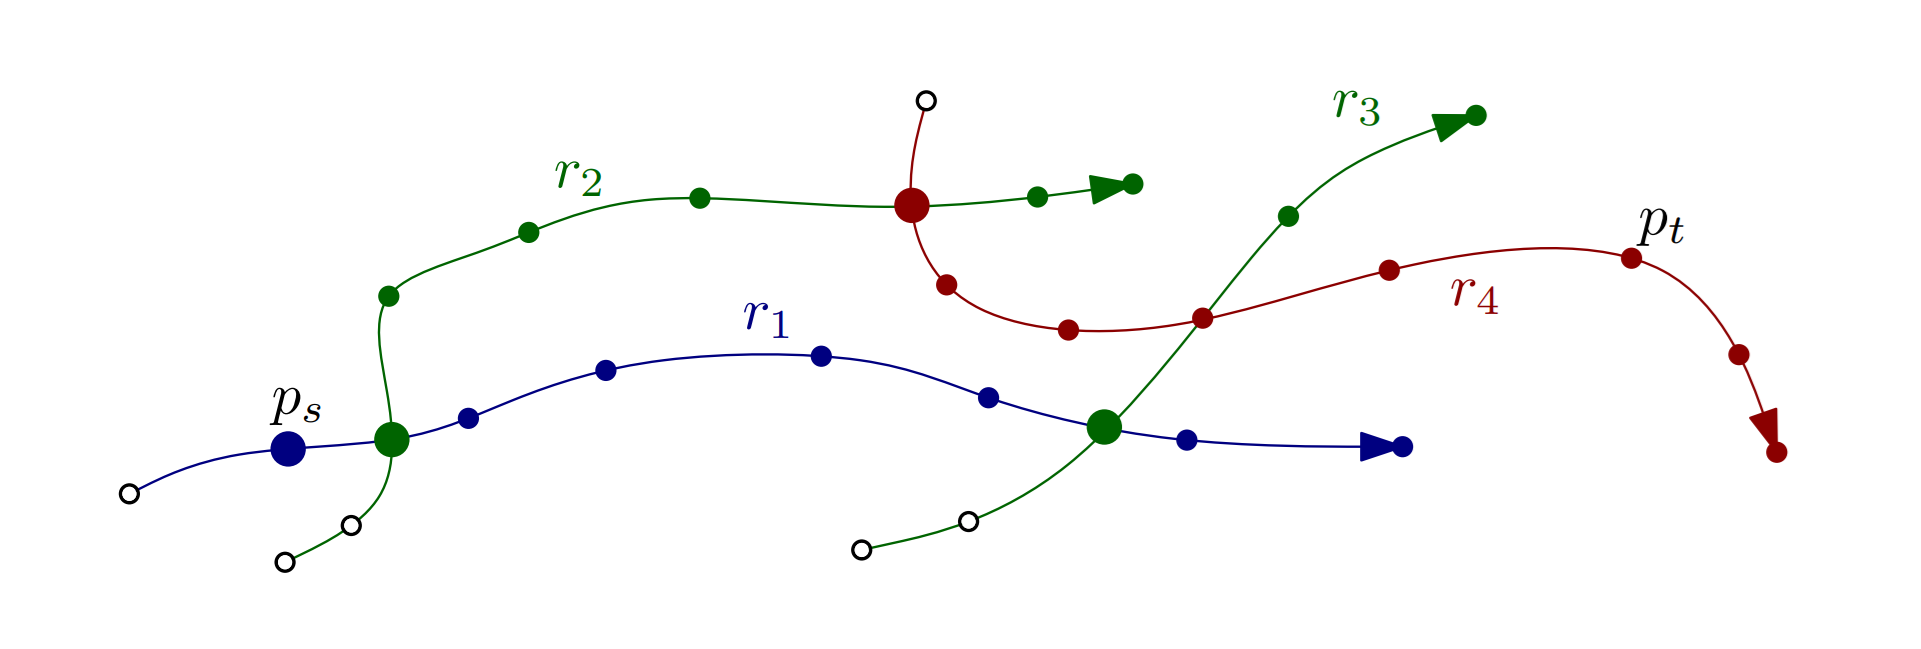
\includegraphics[width=\textwidth]{img/raptor_illustration.png}
    \caption[RAPTOR algorithm illustration]{Scanning routes for a query from p$_s$ to p$_t$. Route r$_1$ is first scanned in round 1, routes r$_2$ and r$_3$ in round 2, and finally, route r$_4$ in round 3. Scanning a route begins at the earliest marked stop (bold). Hollow stops are never visited. Source: \textcite{delling2015raptor}}
    \label{fig:gtfs_scheme}
\end{figure}


After this step is finished, it proceeds to the last step - traversing the transfers. This means that for every marked stop, it goes through all the neighboring stops to where a transfer can be performed and tries to relax their reach times. Once again, if their reach time was improved, it marks them.


This is repeated for a certain number of rounds. The design of the algorithm ensures, that after the n-th round, it has found the best reach time to every stop when using n or less public transit trips. In other words, after the first round, we get the best reach times at stops when only using a single direct trip from the source (and maybe a single transfer to the destination). In the second round, we add the option to transfer once to a different public transit trip and get all the best reach times with a maximum of 2 trips. Same as Dijkstra's algorithm, RAPTOR also finds the best times to all stops within the network, unless it is halted earlier. It can also simply be modified to reconstruct the best connections' path by storing not only the single best reach time, but an array of the best reach times in every round at every stop, together with an array of trips or transfers using which the stop was best reached in every round. Detailed information on the construction of the graph used by the algorithm, along with its pseudocode, can be found in \textcite{delling2015raptor}. 

In our application, we also want to include shared bikes in the search. Using this algorithm, this is actually very simple to do by inserting a new step between the trip traversals and transfer traversals, where we traverse all possible bike trips from every currently marked bike station and try to relax the reach time at the destination.

This algorithm has been shown to be faster than Dijkstra's algorithm and its modifications\cite{delling2015raptor}. It also has the useful feature of providing for every stop the best connections with every possible (and useful) number of trips. For example, if the destination stop can be reached with 0 transfers in 30 minutes, with 1 transfer in 25 minutes and with 2 transfers in 20 minutes, we can recover all of these options and provide them to the user as multiple alternatives. More information on the design of this algorithm and its variations (one of which, the rRAPTOR, our application uses for range searches) can be found in \textcite{delling2015raptor}.

\subsection{Calculating transfers}
\label{subsec:calculating_transfers}

Unfortunately, no data is available on what transfers are possible within Prague's public transit network and how long they take. Due to this, we will have to calculate the transfers ourselves. As we are already using a map router for shared bikes routing, we have the option of using this for walking transfers as well. However, the number of stops within the network is significantly higher than the number of bike stations and these computations would take an extreme amount of time. Additionally, we would also need to store this calculated distance data somewhere and the amount of space it would take up would be very large as well.

Another option is to use a constant global transfer time. This would obviously be very easy to implement, but there are also significant drawbacks to this approach. Mainly, we want our application to support transfers of a wide range of lengths (in particular, we support transfers of up to 750m of length, which turned out to be a great compromise between not having to process too many transfers and providing opportunities for as many time-improving transfers as possible). A constant transfer time could never account for both transfers that may be 0 or just a few meters long and transfers that are upwards of 500m long. Thus, we didn't go with this approach.

The approach we chose is to calculate the straight-line distance between every pair of stops and use this value to approximate the transfer's length and time. Obviously this value will almost never be exact, but it provides us with enough information to make an approximation of the actual length (by using these straight-line distances with a constant multiplier like 120\%).

When using the straight-line approach however, we face an issue in places where there are pairs of stops that are near each other, but it is not actually possible to transfer between them. An example of this would be stops on opposite sides of a river, railway track or a highway. To solve this issue without having to perform expensive map routing calculations, we prepared two simple files describing coordinate lines that may not be crossed by any transfer. First, we specify coordinate points in the \texttt{forbidden\_transfer\_points.csv} file and then describe lines between them in the \texttt{forbidden\_transfer\_points.csv} file, which cannot be crossed during a transfer. In Prague, most of these typically correspond to a river's path, a railway or a significant vertical drop. As our application is only targeted at Prague, there is no issue with managing these small files manually and adding new lines when necessary, as the number of such places is low, thanks to the city's street network being very dense and interconnected.

\subsection{Calculating bike routes}

As was already explained earlier, we will use a third-party library to implement bike routing. This is because for bike trips, which can be upwards of 4 kilometers long, the straight-line approach no longer gives us great approximations of the trips' length, as at that length, the actual shortest route's length may deviate significantly from the calculated straight-line approximation. Same as for the transfers, a constant global bike trip time makes no sense either. Due to all this, we will need to calculate the actual routes between the bike stations. 

We could theoretically use an external third-party API that provides this functionality, however these APIs are typically paid and are not effective for calculating such a large amount of trips. We could also implement a solution ourselves, however that would mean implementing a whole new application, the size of which would far exceed the scope of our project. Thus, we settled on using a library that was designed for this purpose.

